\documentclass[10pt,a4paper]{article}
\usepackage[margin=22mm]{geometry}
\usepackage[T1]{fontenc}
\usepackage{lmodern,amsmath,amssymb,booktabs,graphicx,tikz,hyperref,fvextra}
\usetikzlibrary{arrows.meta,positioning,calc,decorations.pathmorphing}
\definecolor{ink}{RGB}{20,53,78}
\hypersetup{colorlinks=true,urlcolor=ink,linkcolor=ink}
\setlength{\parindent}{0pt}
\setlength{\parskip}{5pt}
\emergencystretch=3em

\title{\color{ink}Gain selection with a third-order actuator}
\author{}
\date{Original learning collection -- November 2026}
\begin{document}
\begin{center}{\LARGE\color{ink}Gain selection with a third-order actuator}\\[5pt]{\small Original learning collection -- November 2026}\end{center}

\textbf{Evidence note.} Original teaching scenario. Numerical parameters are deliberately chosen for learning. All generated data and curves are synthetic; no physical measurement is asserted.
\section{Design brief}
A normalized actuator has $G(s)=1/[s(s+2)(s+6)]$ under unity negative feedback with proportional gain $K>0$. Derive the strictly stable gain interval using Routh--Hurwitz, the imaginary-axis crossing and real-axis breakaway. Simulate $K=12$, $60$ and $100$ to compare regulation and instability. A short time plot alone is not a stability test.
\section{Physical system}
\begin{center}\resizebox{\ifdim\width>.98\linewidth.98\linewidth\else\width\fi}{!}{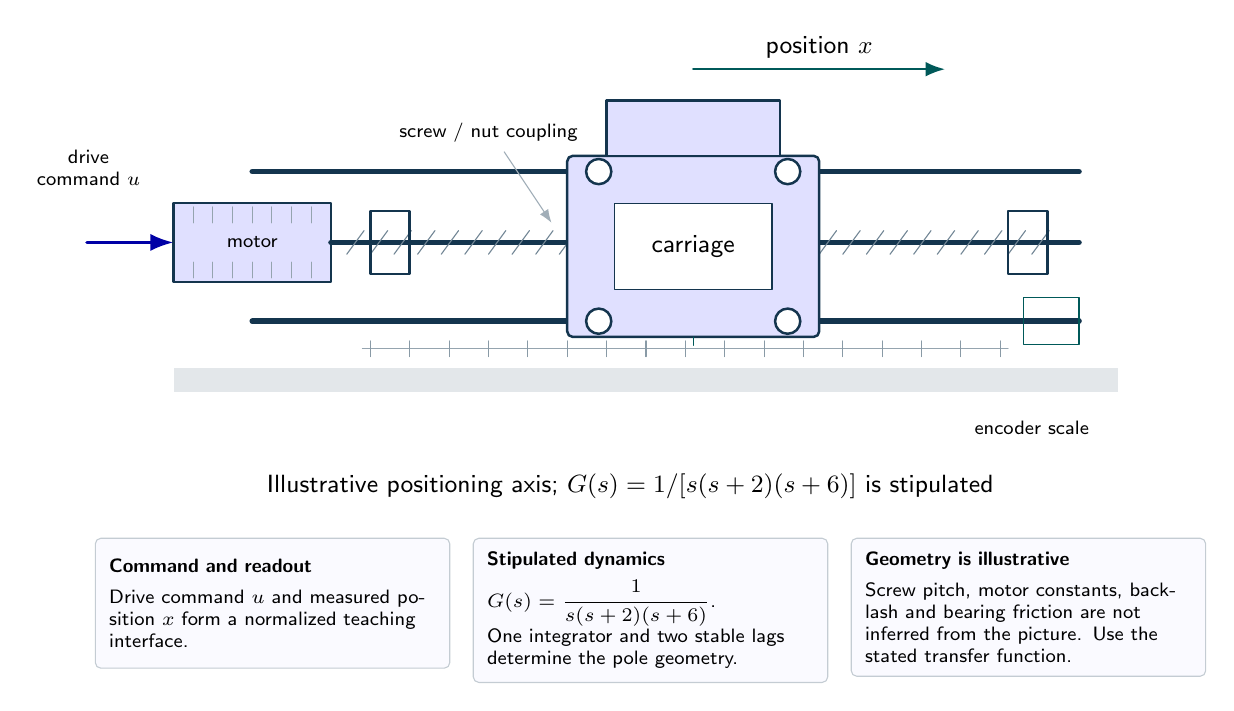
\begin{tikzpicture}[
font=\sffamily\small,>=Latex,line cap=round,line join=round,
wall/.style={draw=ink,line width=1.2pt,fill=blue!5},
water/.style={fill=cyan!25,draw=none},
metal/.style={draw=ink,fill=blue!12,line width=.9pt},
flow/.style={->,draw=blue!65!black,line width=1.2pt},
heat/.style={->,draw=orange!85!black,line width=1.1pt},
measure/.style={->,draw=teal!70!black,line width=.9pt},
dim/.style={<->,draw=ink!65,line width=.6pt},
spring/.style={draw=ink,decorate,decoration={coil,aspect=.5,segment length=4pt,amplitude=3pt}},
wire/.style={draw=ink,line width=1pt},
lab/.style={align=center,font=\sffamily\small},
smalllab/.style={align=center,font=\sffamily\scriptsize}]

\fill[ink!12](1,.5)rectangle(13,.8);
\draw[ink,line width=2pt](2,1.4)--(12.5,1.4)(2,3.3)--(12.5,3.3);
\draw[metal](1,1.9)rectangle(3,2.9);
\node[smalllab]at(2,2.4){motor};
\draw[ink,line width=2pt](3,2.4)--(12.5,2.4);
\foreach \x in {3.2,3.5,...,12.2}{\draw[ink!60](\x,2.25)--++(.22,.3);}
\draw[metal,rounded corners=2pt](6,1.2)rectangle(9.2,3.5);
\draw[fill=white,draw=ink](6.6,1.8)rectangle(8.6,2.9);
\node[lab]at(7.6,2.35){carriage};
\draw[metal](6.5,3.5)rectangle(8.7,4.2);
\draw[measure](7.6,4.6)--(10.8,4.6)node[midway,above]{position $x$};
\draw[flow](-.1,2.4)--(1,2.4);
\node[smalllab,anchor=east]at(.7,3.35){drive\\command $u$};
\draw[teal!70!black](11.8,1.1)rectangle(12.5,1.7);
\node[smalllab]at(11.9,.05){encoder scale};
\node[lab]at(6.8,-.7){Illustrative positioning axis; $G(s)=1/[s(s+2)(s+6)]$ is stipulated};
% REFINED EQUIPMENT DETAILS

% Guide bearings, screw supports and a scale tied to the carriage coordinate.
\foreach \x in {6.4,8.8}{\draw[metal,fill=white](\x,1.4)circle(.16)(\x,3.3)circle(.16);}
\draw[metal,fill=none](3.5,2)rectangle(4,2.8);\draw[metal,fill=none](11.6,2)rectangle(12.1,2.8);
\draw[ink!45](3.4,1.05)--(11.6,1.05);
\foreach \x in {3.5,4,...,11.5}{\draw[ink!50](\x,.95)--(\x,1.15);}
\draw[teal!70!black,densely dashed](7.6,1.2)--(7.6,1.05);
\foreach \x in {1.25,1.5,...,2.75}{\draw[ink!45](\x,1.95)--(\x,2.15)(\x,2.65)--(\x,2.85);}
\node[smalllab]at(5,3.8){screw / nut coupling};
\draw[ink!40,->](5.2,3.55)--(5.8,2.65);

\node[draw=ink!25,fill=blue!2,rounded corners=2pt,anchor=north west,text width=4.15cm,minimum height=1.65cm,inner sep=5pt,align=left,font=\sffamily\scriptsize]at(0.0,-1.35){\textbf{Command and readout}\\[3pt]Drive command $u$ and measured position $x$ form a normalized teaching interface.};
\node[draw=ink!25,fill=blue!2,rounded corners=2pt,anchor=north west,text width=4.15cm,minimum height=1.65cm,inner sep=5pt,align=left,font=\sffamily\scriptsize]at(4.8,-1.35){\textbf{Stipulated dynamics}\\[3pt]$G(s)=\dfrac{1}{s(s+2)(s+6)}$.\\One integrator and two stable lags determine the pole geometry.};
\node[draw=ink!25,fill=blue!2,rounded corners=2pt,anchor=north west,text width=4.15cm,minimum height=1.65cm,inner sep=5pt,align=left,font=\sffamily\scriptsize]at(9.6,-1.35){\textbf{Geometry is illustrative}\\[3pt]Screw pitch, motor constants, backlash and bearing friction are not inferred from the picture. Use the stated transfer function.};
\end{tikzpicture}
}\par{\small A motorized positioning axis illustrates the role of the integrator and two stable lags. The normalized transfer function is specified as a teaching model; the pictured dimensions do not identify its coefficients.}\end{center}
\section{Characteristic equation}
The unity-feedback denominator is
\[p(s)=s(s+2)(s+6)+K=s^3+8s^2+12s+K.\]
The first column of the Routh array is $1,8,(96-K)/8,K$. Strict stability therefore requires $0<K<96$. At $K=0$ there is a pole at the origin; $K=96$ is a boundary, not a stable maximum.
\section{Imaginary-axis crossing}
At $K=96$, $p(s)=(s+8)(s^2+12)$, so the crossing pair is $s=\pm j\sqrt{12}$. The remaining pole stays at $-8$.
\section{Root-locus geometry}
There are three open-loop poles and no finite zeros. The centroid is $-8/3$ and the asymptote angles are $60$, $180$ and $300$ degrees. Real-axis locus segments are $(-\infty,-6)$ and $(-2,0)$.
Since $K(s)=-s(s+2)(s+6)$, a stationary point satisfies $3s^2+16s+12=0$. The root $(-8+2\sqrt7)/3\simeq-0.9028$ belongs to $(-2,0)$ and is the valid positive-gain breakaway. The other stationary point does not lie on a positive-gain real-axis segment.
\section{Checking the plots}
Use pole real parts to classify each gain before plotting. A finite horizon can conceal instability when an unstable real part is small. For stable positive gains, the integrator in the open loop gives zero constant-reference error, but says nothing about overshoot.
\section{What to learn from the experiment}
An algebraic stability interval provides a guardrail for numerical tuning. The endpoint K=96 must be excluded from strict asymptotic stability.
\section{System sketch}
\begin{center}\resizebox{\ifdim\width>.98\linewidth.98\linewidth\else\width\fi}{!}{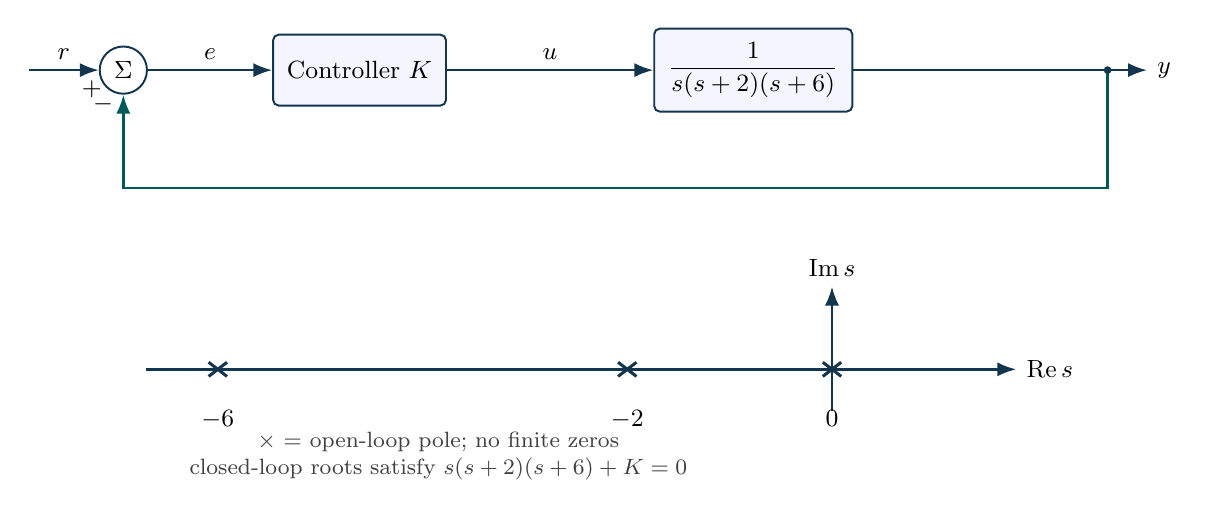
\begin{tikzpicture}[x=1cm,y=1cm,>=Latex,font=\small,
block/.style={draw=ink,fill=blue!4,rounded corners=2pt,minimum height=9mm,align=center,line width=.7pt,inner sep=5pt},
sum/.style={circle,draw=ink,fill=white,minimum size=6mm,inner sep=0pt,line width=.7pt},
sig/.style={->,draw=ink,line width=.85pt},
fb/.style={->,draw=teal!70!black,line width=.85pt},
dist/.style={->,draw=orange!75!black,line width=.85pt},
tap/.style={circle,fill=ink,inner sep=1.4pt},
note/.style={font=\footnotesize,align=center,text=black!75}]

\node[sum](e)at(1,1.8){$\Sigma$};
\node[block](k)at(4,1.8){Controller $K$};
\node[block](p)at(9,1.8){$\dfrac{1}{s(s+2)(s+6)}$};
\draw[sig](-.2,1.8)--node[above]{$r$}node[pos=.9,below]{$+$}(e);
\draw[sig](e)--node[above]{$e$}(k);
\draw[sig](k)--node[above]{$u$}(p);
\draw[sig](p)--(14,1.8)node[right]{$y$};
\draw[fb](13.5,1.8)--(13.5,.3)--(1,.3)--node[pos=.9,left]{$-$}(e);
\fill[ink](13.5,1.8)circle(1.4pt);
\begin{scope}[shift={(10,-2)},x=1.3cm,y=.75cm]
\draw[sig](-6.7,0)--(1.8,0)node[right]{$\operatorname{Re}s$};
\draw[sig](0,-.7)--(0,1.4)node[above]{$\operatorname{Im}s$};
\foreach \v in {-6,-2,0}{\draw[ink,line width=1.1pt](\v-.09,-.12)--(\v+.09,.12)(\v-.09,.12)--(\v+.09,-.12);\node[below=4mm]at(\v,0){$\v$};}
\end{scope}
\node[note]at(5,-3.1){$\times$ = open-loop pole; no finite zeros\\closed-loop roots satisfy $s(s+2)(s+6)+K=0$};

\end{tikzpicture}
}
\par\small\refstepcounter{figure}\label{fig:system}\textbf{Figure \thefigure.} Unity negative feedback and the open-loop pole map. Pole symbols provide the starting geometry for the root-locus exercises.\end{center}
\clearpage
\section{Executed computational evidence}
\VerbatimInput[fontsize=\small,breaklines=true]{results.txt}
\begin{center}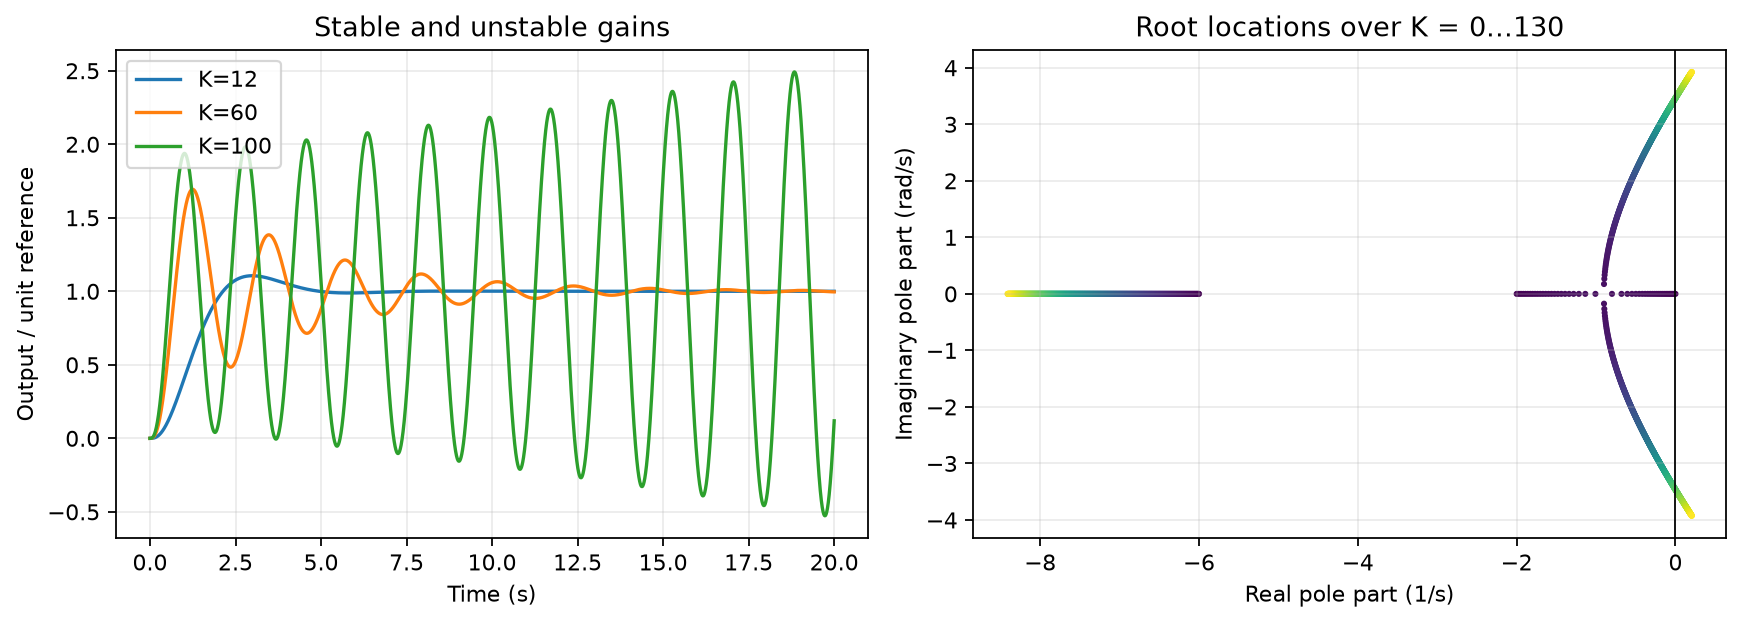
\includegraphics[width=\linewidth,height=.46\textheight,keepaspectratio]{response.png}\end{center}
\paragraph{Method references.}
The equations use standard balance laws and feedback-control methods. Further explanation: \url{https://apmonitor.com/pdc/} and \url{https://fbsbook.org/}. Implementation documentation: \url{https://python-control.readthedocs.io/en/0.10.2/}. See the repository reference catalog for individual topics and videos.
\end{document}
